\documentclass[11pt,twoside,a4paper]{article}
\usepackage{tikz}
\usepackage[english]{babel} %English hyphenation
\usepackage{amsmath} %Mathematical stuff
\usepackage{amsthm}
\usepackage{amssymb}
\usepackage{verbatim}
\usetikzlibrary{arrows}
\usepackage[left=2cm,right=2cm,top=2cm,bottom=2cm]{geometry}

%Hyperreferences in the document. (e.g. \ref is clickable)
\usepackage{hyperref}

%Pseudocode
\usepackage{algorithm}
\usepackage[]{algpseudocode}
%You can also use the pseudocode package. http://cacr.uwaterloo.ca/~dstinson/papers/pseudocode.pdf
%\usepackage{pseudocode}

\usepackage{a4wide,times}
\title{TI2306 Algoritmiek, Lab Assignment 4} %The title, e.g. Algoritmiek Assignment 1
\author{
	Bart Ziengs \\ bziengs \\ 4391799 %Change the author info, Name, netID(, studentnr.)
}
\begin{document}
\maketitle
%\clearpage

\begin{enumerate}
\item If one would choose to compile each function of the three function one would obtain \\
$(10 + 15) + \left((28\times 4 + 10)\right) + \left( (5 \times 6)+10 \right) = 187 $
\item I would define a (minimum) cut $(A,B)$ in which all the to-compile functions $\in A$ en the others $\in B$. In addition, the following variables are used:

$C_f$, \textbf{compile} time for a certain function $f$ \\
$R_f$, \textbf{run} time for a certain function $f$ \\
$T_f$, number of total \textbf{times} a certain function $f$ is called by a function $j$\\
$T_{f \rightarrow j}$, number of total \textbf{times} a certain function $f$ calls a function $j$ \\
$o$, The overhead costs for when a compiled function calls a non-compiled one and vice versa. \\

My formula for what we aim to optimize would be: \\
$ \underbrace{\sum\limits_{f \in A} C_f + \left( R_f \times T_f \right)}_\text{compiled function}  \qquad + \qquad  \underbrace{\sum\limits_{f \in B} R_f \times T_f}_\text{uncompiled functions} \qquad + \qquad \underbrace{\sum\limits_{f \in A,g \in b} T_{f \rightarrow g} \times o}_\text{total overhead} $
\item To properly model this as a network flow problem, I see it like the situation described in section 7.10 of the book. The following would need to hold:
\begin{itemize}
\item Construct for each process a node and add these to a graph.
\item Add an source node $source$ and a sink node $sink$ to the graph.
\item Construct for each node $n$ an edge $\{source,n\}$ with capacity $C_f + R_{f,compiled} \times T_f$ as defined above.
\item Construct for each node $n$ an edge $\{n,sink\}$ with capacity $R_{f,uncompiled} \times T_f$ .
\item Construct for the amount times $c$ that an function $a$ calls $b$ an two edges $\{a,b\}$ and $\{b,a\}$ with capacity $c*o$. Two edges are needed because if you would obtain a minimum cut $(A,B)$ you would need to determine the capacity by summing up all edges that go from $A$ to $B$ so you need a double edge.
\item Now the minimum cut $(A,B)$ can be determined. The capacity of this cut will be the minimal outcome of the formula derived at \textbf{2.}. This is also equal to the maximum possible flow in this specific flow network.
\end{itemize}
\newpage
An example is given in the figure below, this is the situation from question \textbf{1.} and has three functions
\begin{figure}[!h]
\centering
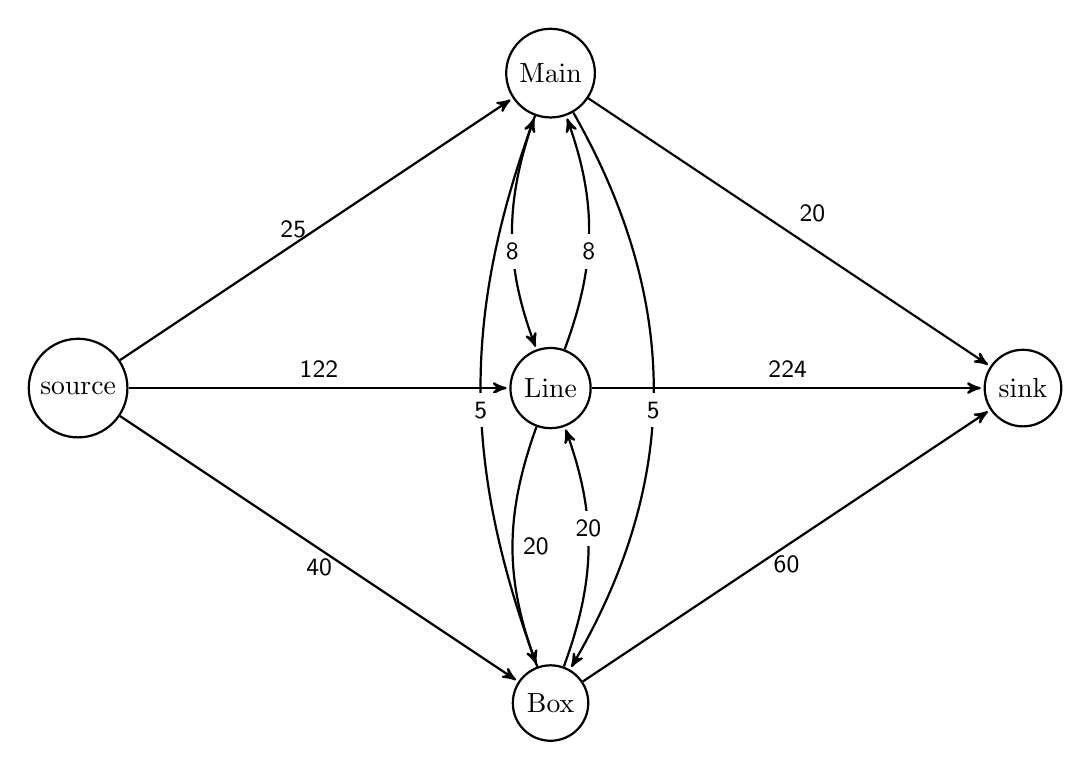
\begin{tikzpicture}[->,>=stealth',shorten >=1pt,auto,node distance=5cm,
                    thick,main node/.style={circle,draw}]
\node[main node] (1) at (0,0){source};
\node[main node] (2) at (6,4) {Main};
\node[main node] (3) at (6,0) {Line};
\node[main node] (4) at (6,-4) {Box};
\node[main node] (5) at (12,0) {sink};
\path[every node/.style={font=\sffamily\small}]

(1) edge node[left]{25} (2)
edge node {122} (3)
edge node[below] {40} (4)
(2) edge[bend right=20] node[below, fill = white]{8}(3)
edge[bend left= 30] node[below, fill = white]{5}(4)
edge node {20}(5)
(3) edge[bend right=20] node[below, fill = white]  {8}(2)
edge[bend right=20] node{20}(4)
edge node{224}(5)
(4)edge node[below]{60}(5)
edge[bend right=20] node[above, fill = white]{20}(3)
edge[bend left = 20] node[below, fill = white]{5}(2)
;

\end{tikzpicture}
\end{figure}
\newline
It can be seen that the minium cut $\left\lbrace\{source\},\{main,line,box\}\right\rbrace$ is equal to 187.
\item The pseudo code is shown below. For each process a node is constructed with the capacities as defined in the previous question. Because the main function is always called once, we need to increment the calls to main with one. Subsequently we can deal with all the function calls, we create two directed edges because this is necessary when you want to calculate the maximum flow. 
		\begin{algorithm}[!h]
		\caption{Minimum run time with maximum flow }
		\label{alg:summation} 
		\begin{algorithmic}[1]
			\State let $g$ be a graph 
			\State add source node $s$ to $g$
			\State add source node $t$ to $g$
			\State
			\For{\textbf{each} function $f$ } 
			\State create a node			
			\State add edge $(s,f)$
			\State add edge $(t,f)$
			\EndFor
			\State
			\State increment the function calls to main with 1
			\State
			\For{\textbf{each} function call from $f$ to $g$ } 
			\State add edge $(f,g)$
			\State add edge $(g,f)$
			\EndFor
			\State
			\State Maximize the flow in $g$
			\State
			\State \textbf{print} the path of the nodes that the maximum flow traverses
			\State \Return $sum$
		\end{algorithmic}
	\end{algorithm}

\item Because the number we want to minimize is: (as stated in \textbf{2.}) \\
$ \sum\limits_{f \in A} C_f + \left( R_f \times T_f \right)  +   \sum\limits_{f \in B} R_f \times T_f + \sum\limits_{f \in A,g \in b} T_{f \rightarrow g} \times o $ \\
And this is equivalent to Maximizing: \\
$ \sum\limits_{f \in B} C_f + \left( R_f \times T_f \right)  +   \sum\limits_{f \in A} R_f \times T_f - \sum\limits_{f \in A,g \in b} T_{f \rightarrow g} \times o $ \\
And that is exactly what we want to achieve.
\item See weblab for 
\item last question.
\end{enumerate}
\begin{thebibliography}{9}
\bibitem{boek}
J. Kleinberg, \' E. Tardos, 
Algorithm Design, 
Pearson Addison Wesley, 
2006.
\bibitem{slides}
\href{https://blackboard.tudelft.nl/webapps/portal/frameset.jsp?tab\_tab\_group\_id=\_10\_1\&url=%2Fwebapps%2Fblackboard%2Fexecute%2Flauncher%3Ftype%3DCourse%26id%3D_45924_1%26url%3D}{Blackboard slides}
\end{thebibliography}
\end{document}
